% ---
% Capa
% ---
\imprimircapa
% ---

% ---
% Folha de rosto
% (o * indica que haverá a ficha bibliográfica)
% ---
\imprimirfolhaderosto*
% ---

% ---
% Inserir a ficha bibliografica
% ---
% http://ficha.bu.ufsc.br/
\begin{fichacatalografica}
	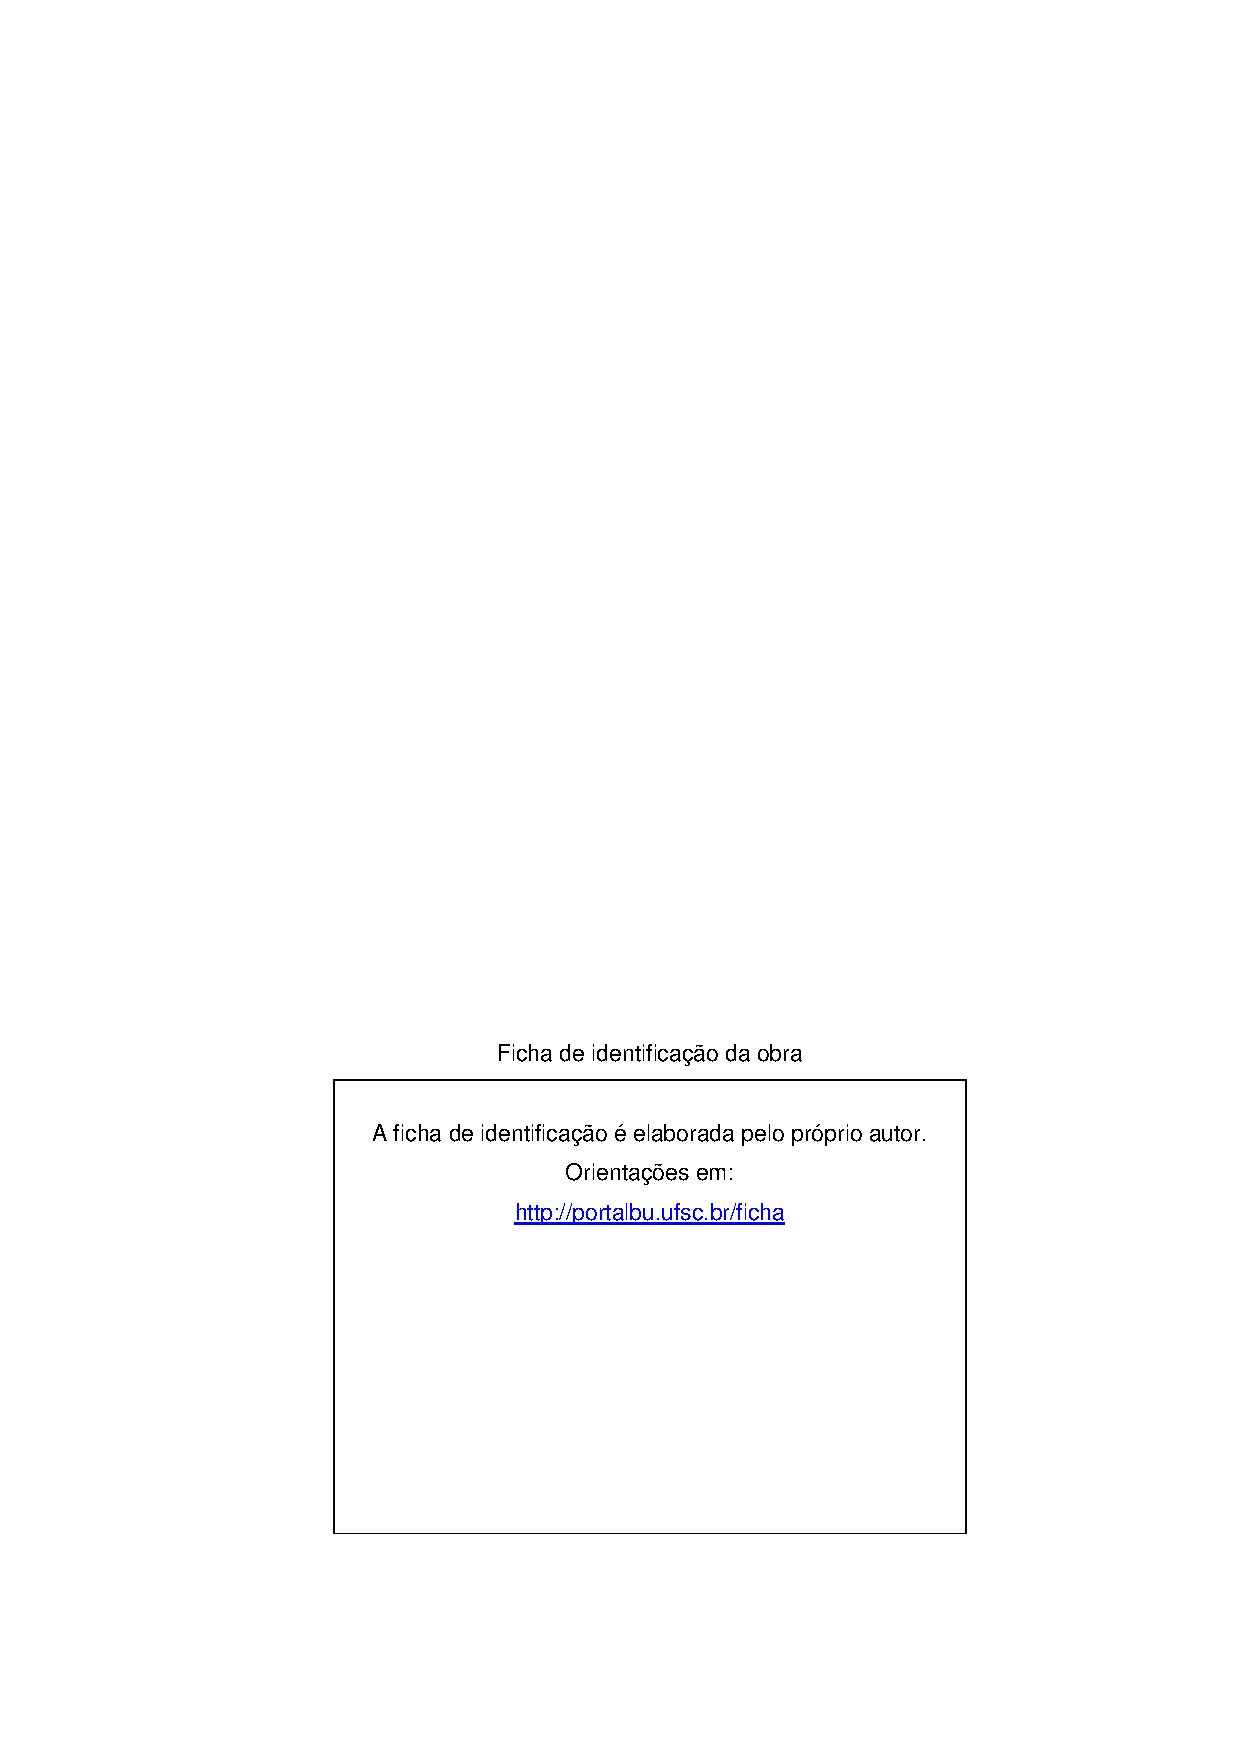
\includepdf{beforetext/Ficha_Catalografica.pdf}
\end{fichacatalografica}
% ---

% ---
% Inserir folha de aprovação
% ---
\begin{folhadeaprovacao}
	\OnehalfSpacing
	\centering
	\imprimirautor\\%
	\vspace*{10pt}		
	\textbf{\imprimirtitulo}%
	\ifnotempty{\imprimirsubtitulo}{:~\imprimirsubtitulo}\\%
	%		\vspace*{31.5pt}%3\baselineskip
	\vspace*{\baselineskip}
	%\begin{minipage}{\textwidth}
	% ~do~\imprimirprograma~do~\imprimircentro~da~\imprimirinstituicao~para~a~obtenção~do~título~de~\imprimirformacao.
	Este~\imprimirtipotrabalho~foi julgado adequado para obtenção do Título de “\imprimirformacao” e aprovado em sua forma final pelo~\imprimirprograma. \\
		\vspace*{\baselineskip}
	\imprimirlocal, \imprimirdata. \\
	\vspace*{2\baselineskip}
	\assinatura{\OnehalfSpacing\imprimircoordenador \\ \imprimircoordenadorRotulo~do Curso}
	\vspace*{2\baselineskip}
	\textbf{Banca Examinadora:} \\
	\vspace*{\baselineskip}
	\assinatura{\OnehalfSpacing\imprimirorientador \\ \imprimirorientadorRotulo}
	%\end{minipage}%
	\vspace*{\baselineskip}
	\assinatura{Prof.(a) xxxx, Dr(a).\\
	Avaliador(a) \\
	Instituição xxxx}

	\vspace*{\baselineskip}
	\assinatura{Prof.(a) xxxx, Dr(a).\\
	Avaliador(a) \\
	Instituição xxxx}


\end{folhadeaprovacao}
% ---

% ---
% Dedicatória
% ---
\begin{dedicatoria}
	\vspace*{\fill}
	\noindent
	\begin{adjustwidth*}{}{5.5cm}     
		Este trabalho é dedicado aos meus colegas de classe e aos meus queridos pais.
	\end{adjustwidth*}
\end{dedicatoria}
% ---

% ---
% Agradecimentos
% ---
\begin{agradecimentos}
	Inserir os agradecimentos aos colaboradores à execução do trabalho. 
	
	Xxxxxxxxxxxxxxxxxxxxxxxxxxxxxxxxxxxxxxxxxxxxxxxxxxxxxxxxxxxxxxxxxxxxxx. 
\end{agradecimentos}
% ---

% ---
% Epígrafe
% ---
\begin{epigrafe}
	\vspace*{\fill}
	\begin{flushright}
		\textit{``Texto da Epígrafe.\\
			Citação relativa ao tema do trabalho.\\
			É opcional. A epígrafe pode também aparecer\\
			na abertura de cada seção ou capítulo.\\
			Deve ser elaborada de acordo com a NBR 10520.''\\
			(Autor da epígrafe, ano)}
	\end{flushright}
\end{epigrafe}
% ---

% ---
% RESUMOS
% ---

% resumo em português
\setlength{\absparsep}{18pt} % ajusta o espaçamento dos parágrafos do resumo
\begin{resumo}
	\SingleSpacing
	O monitoramento da qualidade do ar tem experimentado uma mudança de paradigma a partir da incorporação de sensores de baixo custo às aplicações de medição de gases. Estes novos equipamentos têm potencial para aumentar a resolução espaço-temporal dos dados de poluentes e complementar as aplicações de monitoramento de referência. Todavia, esses dispositivos ainda devem alcançar níveis de confiabilidade apropriados para serem utilizados de forma estendida. A literatura reporta a aplicação de vários modelos de calibração baseados em técnicas de aprendizado de máquina que têm melhorado a qualidade das medições. No presente trabalho apresenta-se a iniciativa CLEAN (Collaborative Low-cost Environmental Air quality Network) que consiste em uma rede colaborativa para o monitoramento de baixo custo da qualidade do ar. CLEAN disponibiliza um marco de trabalho para acelerar e facilitar o desenvolvimento e a diversificação de aplicações de monitoramento de baixo custo da qualidade do ar. Os componentes da inciativa e suas contribuições na área de monitoramento da qualidade do ar são apresentadas e descritas em detalhe no corpo desta tese. Dentro do contexto da pesquisa foram desenvolvidos monitores de baixo custo que foram incorporados à rede CLEAN. Um dos dispositivos foi instalado junto a uma estação de monitoramento de referência da qualidade do ar para validação e calibração das leituras do instrumento de baixo custo. O equipamento foi instalado por um período de 6 meses durante os quais foram armazenadas em cartão físico e banco de dados remoto as leituras de \acrshort{co}, \acrshort{o3}, \acrshort{no2}, \acrshort{so2}, \acrshort{mp10} e temperatura. Os dados adquiridos foram pré-processados e analisados antes de calibrar os equipamentos. Em geral observaram-se frequentes perturbações nos valores de linha base dos sensores que inviabilizaram boa parte dos dados. Em particular as leituras de \acrshort{so2} e \acrshort{no2} se mostraram ruidosas e com alterações muito frequentemente na linha base e portanto esses dados foram descartados. As leituras de \acrshort{co}, \acrshort{o3} e \acrshort{mp10} mostraram uma correlação estatisticamente significativa com a temperatura, em especial o \acrshort{o3} que chegou a apresentar coeficientes de Spearman e Kendall de 0.8 e 0.7 respectivamente. Com relação às medições de referência, as leituras dos sensores de baixo custo mostraram uma correlação estatisticamente significativa. Os testes realizados evidenciaram os melhores resultados nos sensores eletroquímicos quando a temperatura foi considerada nos modelos de calibração com valores de R2 de até 0.4 com uma regressão utilizando uma rede neural Perceptron Multicamadas para as leituras de \acrshort{o3}. Observou-se uma melhoria significativa nos resultados da calibração quando as leituras dos sensores dos 3 poluentes foram consideradas para inferir as concentrações de referência. Por exemplo, para o \acrshort{co}, que gerou valores negativos de R2 quando considerado individualmente, conseguiu um R2 máximo de 0.1 quando consideradas também as leituras de \acrshort{o3} e \acrshort{mp10} e aplicada uma regressão pelo método k vizinhos mais próximos.
	
	\textbf{Palavras-chave}: Monitoramento da qualidade do ar, aprendizado de máquina, calibração, sensores eletroquímicos, sistemas embarcados
\end{resumo}

% resumo em inglês
\begin{resumo}[Abstract]
	\SingleSpacing
	\begin{otherlanguage*}{english}
		Resumo traduzido para outros idiomas, neste caso, inglês. Segue o formato do resumo feito na língua vernácula. As palavras-chave traduzidas, versão em língua estrangeira, são colocadas abaixo do texto precedidas pela expressão “Keywords”, separadas por ponto.
		
		\textbf{Keywords}: Keyword 1. Keyword 2. Keyword 3.
	\end{otherlanguage*}
\end{resumo}

%% resumo em francês 
%\begin{resumo}[Résumé]
% \begin{otherlanguage*}{french}
%    Il s'agit d'un résumé en français.
% 
%   \textbf{Mots-clés}: latex. abntex. publication de textes.
% \end{otherlanguage*}
%\end{resumo}
%
%% resumo em espanhol
%\begin{resumo}[Resumen]
% \begin{otherlanguage*}{spanish}
%   Este es el resumen en español.
%  
%   \textbf{Palabras clave}: latex. abntex. publicación de textos.
% \end{otherlanguage*}
%\end{resumo}
%% ---

{%hidelinks
	\hypersetup{hidelinks}
	% ---
	% inserir lista de ilustrações
	% ---
	\pdfbookmark[0]{\listfigurename}{lof}
	\listoffigures*
	\cleardoublepage
	% ---
	
	% ---
	% inserir lista de quadros
	% ---
	\pdfbookmark[0]{\listofquadrosname}{loq}
	\listofquadros*
	\cleardoublepage
	% ---
	
	% ---
	% inserir lista de tabelas
	% ---
	\pdfbookmark[0]{\listtablename}{lot}
	\listoftables*
	\cleardoublepage
	% ---
	
	% ---
	% inserir lista de abreviaturas e siglas (devem ser declarados no preambulo)
	% ---
	% \imprimirlistadesiglas
	% ---
	
	% ---
	% inserir lista de símbolos (devem ser declarados no preambulo)
	% ---
	% \imprimirlistadesimbolos
	% ---
	\printglossary[title=Lista de Siglas, toctitle=Lista de siglas]
    \printglossary[type=\acronymtype,title=Lista de Símbolos, toctitle=Lista de símbolos]

	% ---
	% inserir o sumario
	% ---
	\pdfbookmark[0]{\contentsname}{toc}
	\tableofcontents*
	\cleardoublepage
	
}%hidelinks
% ---